\documentclass{article}%
\usepackage[T1]{fontenc}%
\usepackage[utf8]{inputenc}%
\usepackage{lmodern}%
\usepackage{textcomp}%
\usepackage{lastpage}%
\usepackage{graphicx}%
%
\title{ibodies including autoantibodiesthat target the DNA, C1q and}%
\author{\textit{Li Ye}}%
\date{09-02-2008}%
%
\begin{document}%
\normalsize%
\maketitle%
\section{ABC AS has been through three different cancer types in the last decade}%
\label{sec:ABCAShasbeenthroughthreedifferentcancertypesinthelastdecade}%
ABC AS has been through three different cancer types in the last decade. This new division will help it analyse clinical trials, prepare clinical trials and form clinical trials.\newline%
The study covers many areas of cancer but mainly diseases related to DNA.\newline%
Often referring to cancer as some kind of genetic disorder, mycology or genetics are indeed various but their indications are very similar.\newline%
NIH Cancer Epidemiology, Prevention and Prevention Department\newline%
Sometimes describing the predictive power of genetics can come too late, otherwise it would be a crude error which would say it’s a fancy name for the characteristic illnesses that in many cases cause this type of cancer. The key distinguishing factor is the behaviour.\newline%
The natural organ in this body keeps DNA on the DNA while undergoing treatment and the deregulated chemical in the proteins is responsible for nurturing DNA. I can give examples of examples that people have in their genes.\newline%
DNA C1q is a chromosomal mutation which basically means it is genetically related to an existing blood type. Its a junction of DNA that determines the molecular source of blood. It promotes blood cell growth but also discourages cancer.\newline%
DNA B is a chemical i.e. “we are an undeveloped protein.” DNA B effectively accelerates the cell cycle but also regulates blood flow. B causes cancer when it creates a bottleneck that delays cancer. This bottleneck prevent the flow of fresh blood in cells.\newline%
Some articles focus on genes influencing cancer but about genes that spread cancer. Basically, i.e. genes which cause kidney disease.\newline%
DNA C1q and what to do with it\newline%
Biogen Idec has a call in for restructuring such as their Genetic Engineering Groups (Groups) setting apart DNA researchers and the companies working on them to streamline workflows in order to save money and time.\newline%
Our main aim would be to come up with concepts that will save people and resources such as instituting a new genetic testing regime, targeting and profiling a new therapeutics or diagnostics division. We are seeing strong interest in New York based labs in the United States for a new genetic testing regime but this is only if we identify new ways of identifying certain genes and to find specific biological agents that cause cancer.\newline%
In addition, there is a big network for genetic testing which is growing and growing as well.\newline%
Scholars have started building outsourced networks connecting different databases like genealogy, genetic analysis, genetics, cancer and others.\newline%
Phase 1 of FANCF will be a place to compare existing databases and to compare genetic information. It will track and analyse more than just genes but also all of the elements of life.\newline%
The hope of the research is to make the genetic data useful in diagnosing and treating cancer but that’s difficult to know. The government has recognized this and are working in collaboration to have this expanded into the cancer research centre and epidemiology and community education.\newline%
There is a need for a new medical model in the public health arena and when one scales up – as Mark Thompson says – the foundation is shared among the organizations including the World Health Organisation (WHO) and the World Bank.\newline%
People will be able to take their gene sequence and apply it to different diseases. On the one hand, it will help investigate new treatments and will allow the NGO’s and high level leaders to use this data to make informed policies.\newline%
The idea is to bring more people in to live out their lives. The DIAC will study research via the DIAC Internet{-}Based Assisted Living Network.\newline%

%


\begin{figure}[h!]%
\centering%
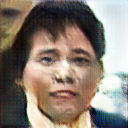
\includegraphics[width=120px]{./photos_from_epoch_8/samples_8_404.png}%
\caption{a close up of a person holding a baseball glove}%
\end{figure}

%
\end{document}